\chapter{Introduction}
\label{ch:intro}

%1. Introduction to how things work visualization
\textit{How things work} visualizations have been used as an efficient method to illustrate how a wide range of systems work.
This technique usually involves displaying where each part is in relation to the system, showing how force is transmitted from one piece to the next or animating motion. 
In order to perform this task a range of visual transformations are used, such as viewing the system from different angles, zoom degrees,  transparency levels, as well as displaying only a subset of the parts.
Generating material of this sort typically involves manual methods, usually in the form of an expert drawing each illustration by hand or composing a fixed animation using specific software.

\begin{figure}[htbp]
        \centering
        \begin{subfigure}[b]{0.3\textwidth}
                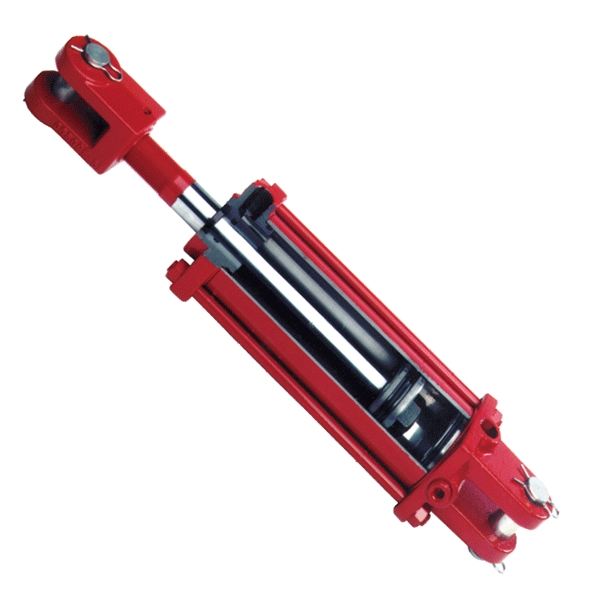
\includegraphics[width=\textwidth]{images/h_pump}
                \caption{Cross section of a typical hydraulic cylinder.}
                \label{fig:h_pump}
        \end{subfigure}%
        ~ %add desired spacing between images, e. g. ~, \quad, \qquad, \hfill etc.
          %(or a blank line to force the subfigure onto a new line)
        \begin{subfigure}[b]{0.3\textwidth}
                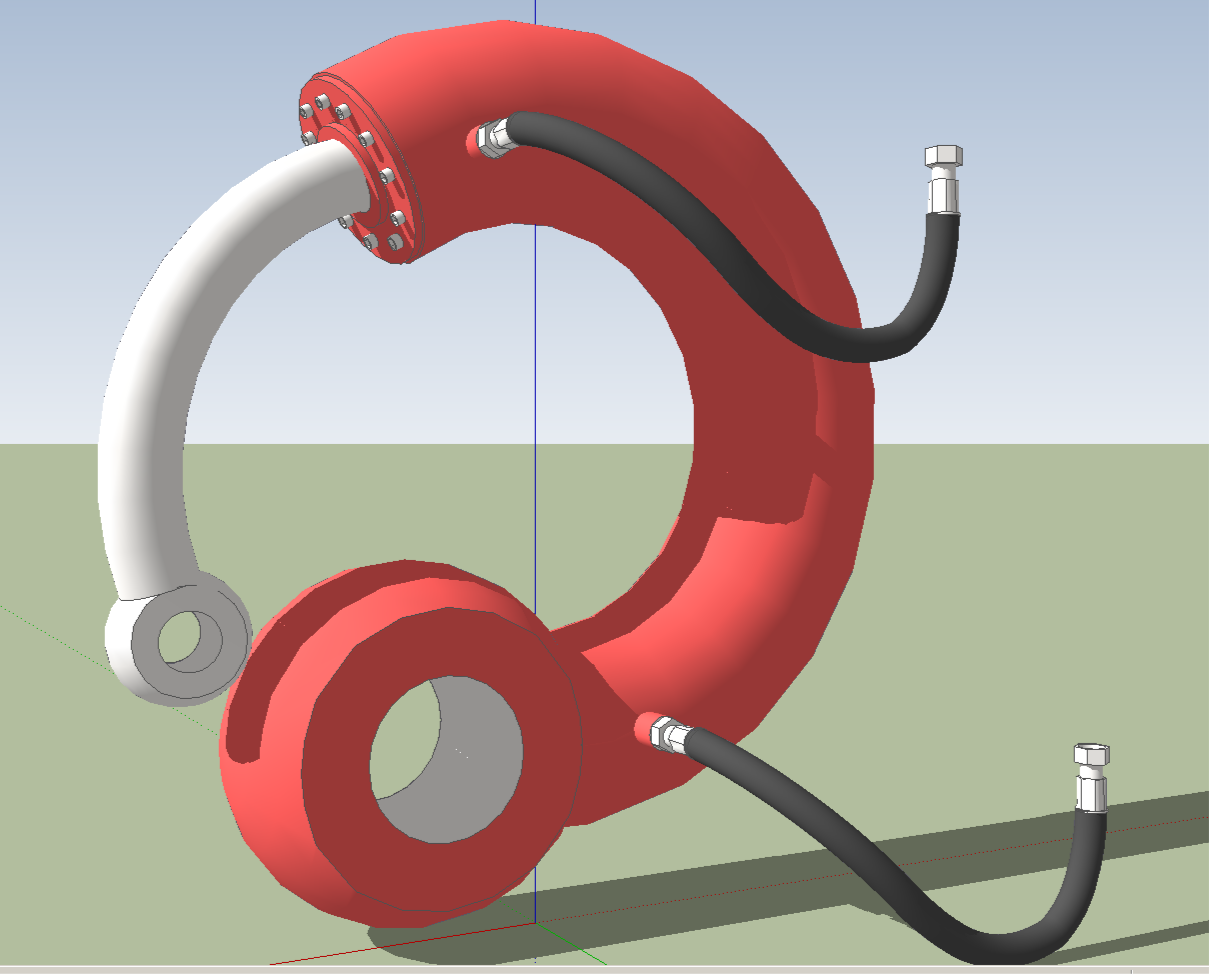
\includegraphics[width=\textwidth]{images/piston}
                \caption{A 3D model of a hydraulic piston.}
                \label{fig:pistonModel}
        \end{subfigure}
        ~ %add desired spacing between images, e. g. ~, \quad, \qquad, \hfill etc.
          %(or a blank line to force the subfigure onto a new line)
        \begin{subfigure}[b]{0.3\textwidth}
                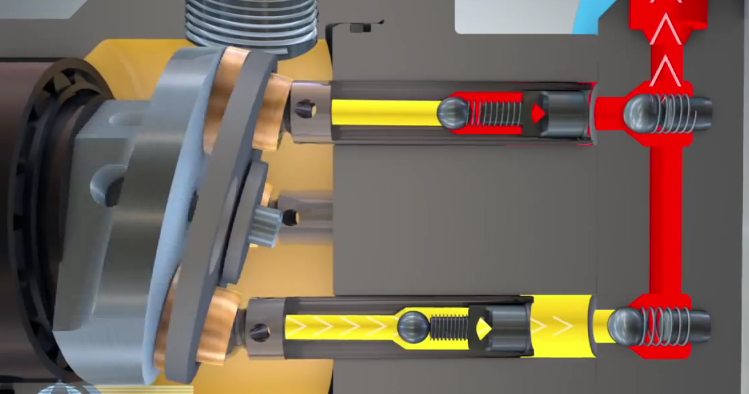
\includegraphics[width=\textwidth]{images/cylinder_animation}
                \caption{Frame of manually generated animation of a hydraulic pump.}
                \label{fig:cylinder_animation}
        \end{subfigure}
        \caption{Overview of the intented workflow}\label{fig:AnimOverview}
\end{figure}

%2. Introduction to hydraulics mechanisms
Hydraulic machinery is commonly used in our everyday lives, for instance lifting cars with jacks, rams on excavators or gerotors to control fuel intake, as shown in Figure~\ref{fig:h_pump}.
Their popularity is based on their faculty to transmit a force or torque multiplication independently of the distance between input and output.
Moreover, they operate silently, can wield force accurately and have the ability to apply torque multiplication easily.
A typical hydraulic equipment has a contained incompressible fluid that becomes pressurised when a force is applied to it, as shown in Figures~\ref{fig:hydraSimpleDiag} and \ref{fig:hydraSimpleCircuit}.
Then that force is transmitted to the other end of the fluid.
In order to grasp how the whole system works, it is essential to understand how the pressure is directed and how it interacts with other parts in the machinery. 
Therefore, to illustrate the general process, the spatial configuration of each part in the system must be unveiled, as well as the chain of motions, that takes place within the gears and the hydraulic fluids.

%3. What are the visualization/illustration techniques for hydraulics mechanisms, refer to SIG10 gear paper.
In order to generate \textit{How things work} visualizations, we first need a 3D model of the physical machinery that we will be working with, as shown in Figure~\ref{fig:pistonModel}.
There are some common visualisation and illustration techniques used for hydraulic machinery, as shown in Figure~\ref{fig:cylinder_animation}.
\textbf{Motion arrows} can point out how the solid parts move and they also indicate fluid flow movement.
\textbf{Frame sequences} display key frames in complex motions and they can highlight temporal interactions between the parts.
\textbf{Animations} are a useful tool to show the behaviour of highly dynamic systems, for example when an excessive number of frame sequences are needed in a particularly complicated motion.

%4. Why this is difficult (designer need to understand force, flow movement, cannot change viewpoint, etc.)
Generating visualisations and illustrations for hydraulic machinery is challenging for designers.
They must understand in detail what forces are generated when parts interact with each other and what kind of flow movements are entailed.
Furthermore, it is impossible to change the viewpoint to explore the object from different angle when 2D illustrations are used.
Moreover, when animations for hydraulic visualizations are generated, they are infrequently updated, since manual animation is a costly and time consuming task.


\begin{figure}[htbp]
        \centering
        \begin{subfigure}[b]{0.3\textwidth}
                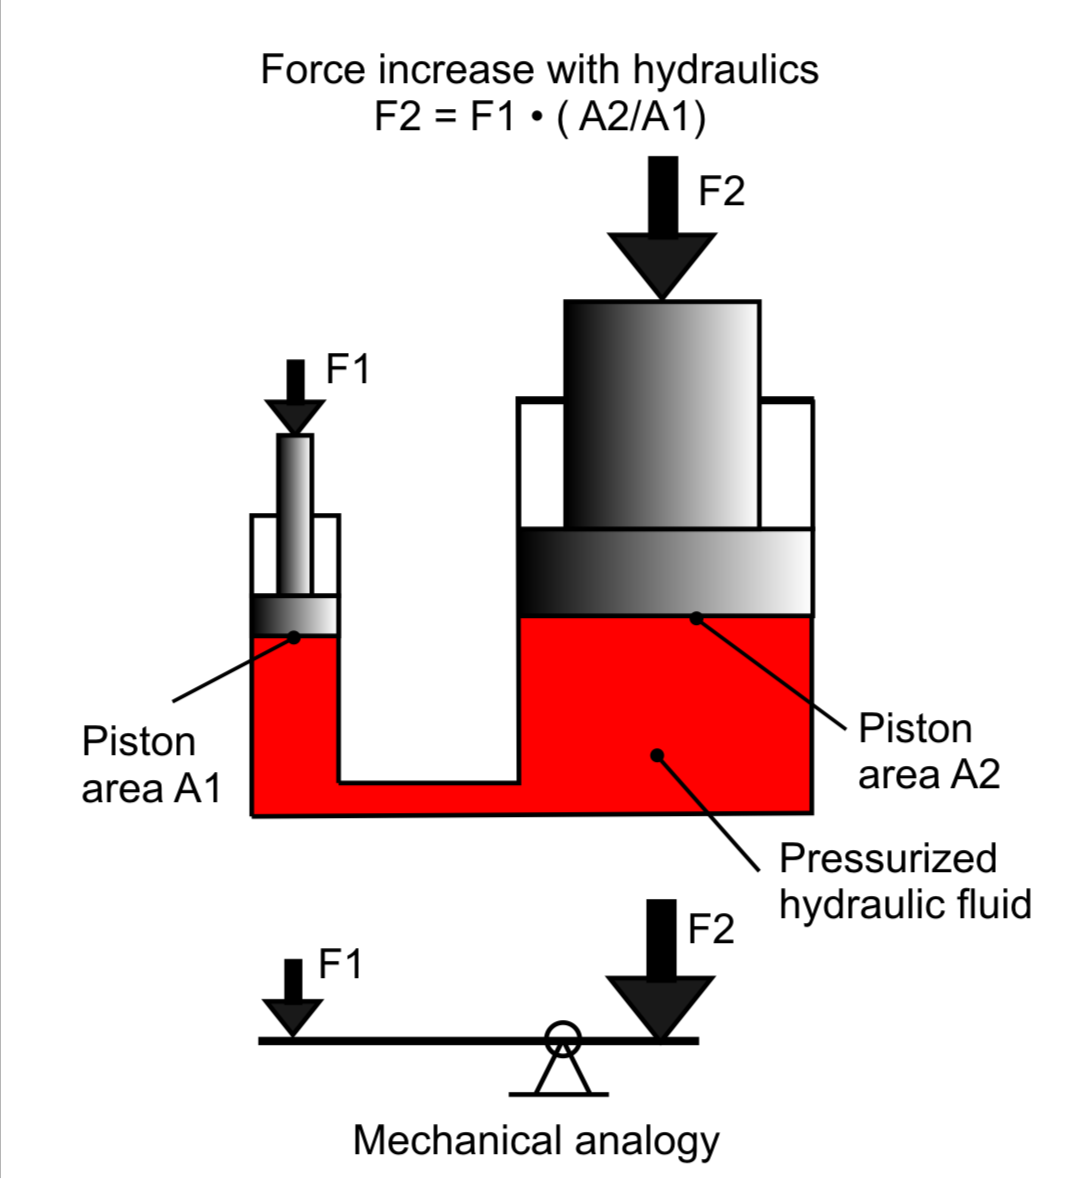
\includegraphics[width=\textwidth]{images/Hydraulic_Force_Torque}
                \caption{Simple hydraulic diagram with a mechanical analogy for easier understanding.}
                \label{fig:hydraSimpleDiag}
        \end{subfigure}%
        \qquad %add desired spacing between images, e. g. ~, \quad, \qquad, \hfill etc.
          %(or a blank line to force the subfigure onto a new line)
        \begin{subfigure}[b]{0.4\textwidth}
`                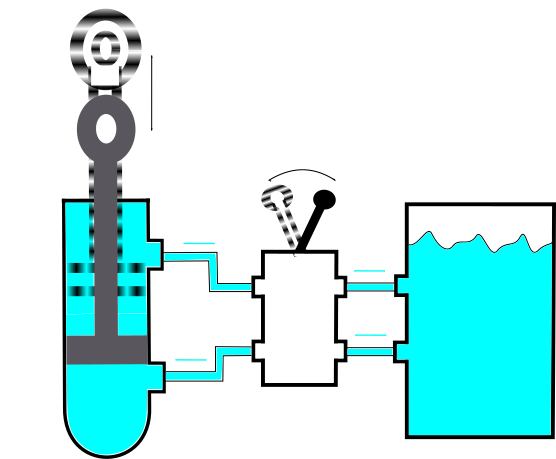
\includegraphics[width=\textwidth]{images/pump_internal}
                \caption{Simplified hydraulic circuit for a hydraulic cylinder.}
                \label{fig:hydraSimpleCircuit}
        \end{subfigure}
        \caption{Sample diagrams for hydraulic mechanisms.}\label{fig:HydraulicDrawings}
\end{figure}

%5. Current status in the research field (mechanical assemblies SIG10, flow systems SIG ASIA 11, maybe some others? No need reference, just some general  discussion, since we have related work part also. And these work cannot handle hydraulics system)
There has been some work done on automatically generating illustrations and visualizations on mechanical assemblies.
Nevertheless, it has been restricted to gear to gear interaction only, i.e. solid parts interacting with other solid parts, as gear movement can be inferred using symmetry information, whereas work on fluid simulation and visualization has not been applied to hydraulic equipment.
Simulations is this field are usually designed to either generate complex visualizations, for engineering purposes, or to produce visually plausible, yet not physically accurate results for animation or games.

%6. Our aim (analysis + visualization, with some description, refer to SIG10 gear paper)
This research proposal aims to introduce a method for generating \textit{How things work} illustrations for hydraulic machinery.
Simulations would be used to generate explanatory depictions of hydraulic machinery, these illustrations would help users understanding how this kind of equipment works.

%7. Summarize our contribution
In summary, the main contributions would be:
\begin{itemize}
\item An application for creating how things works illustration for 3D hydraulic machinery models.
\item A method for detecting motion and interaction of fluid in the model parts.
\item An algorithm to automatically generate illustrations with motion arrows and key frame sequences.
\end{itemize}